% This file should be replaced with your file with an appendices (headings below are examples only)

% Placing of table of contents of the memory media here should be consulted with a supervisor
\chapter{Contents of the included storage media}
\dirtree{%
.1 /.
.2 thesis ---- thesis documentation source codes.
.2 xvasil03.pdf ---- Thesis document.
.2 src ---- source codes.
.3 enoss ---- ENOSS repository.
.4 benchmark ---- benchmark results.
.5 expr1 ---- benchmark resuls for experiment 1.
.5 expr2 ---- benchmark resuls for experiment 2.
.5 expr3 ---- benchmark resuls for experiment 3.
.5 k8s ---- k8s sources used for benchmarking.
.4 demo ---- OpenIO SDS and OpenStack Swift demo with enabled ENOSS.
.4 enoss ---- ENOSS source codes.
.5 enoss.py ---- ENOSS middleware.
.5 destinations ---- destination handlers.
.5 payloads ---- payload handlers.
.5 filter\_rules ---- filter rule handlers.
.4 etc/swift/enoss ---- configuration.
.4 test ---- ENOSS tests.
.5 functional.
.5 unit.
.4 examples ---- Several examples of notifications configurations.
.3 mqtt-to-beanstalkd ---- source codes for MinIO proxy from MQTT to Beanstalkd.
}

\chapter{Repository and Usage Guide}
ENOSS repository is publicly avaliable at the Github {\url{https://github.com/xvasil03/enoss}}.

\textbf{ENOSS demo} is stored in \texttt{enoss/demo}. Demo contains following containers:
\begin{itemize}
    \item \textbf{Beanstalkd listener} - contains beanstalkd service, receives notifications from OpenIO SDS and Swift and prints then to stdout (docker logs).
    \item \textbf{ENOSS Swift} - container with OpenStack Swift with enabled ENOSS. Can publish notifications to beanstalkd. After container init runs UNIT and FUNCTIONAL ENOSS tests.
    \item \textbf{ENOSS OpenIO} - container with OPENIO SDS with enabled ENOSS. Can publish notifications to beanstalkd.
    \item \textbf{Demo worker} - waits 2 minutes for other containers to initialize then runs demo scripts \texttt{enoss/demo/demo\_openio.sh} and \texttt{enoss/demo/demo\_swift.sh} Demo scripts will enable notifications on specific container, read stored configuration from object storage, and then create event which will trigger notification. Connect to this container and communicate with OpenStack Swift using hostname \texttt{swift-service} and with OpenIO SDS using hostname \texttt{openio-service}.
\end{itemize}
Run demo using \textbf{\texttt{docker-compose up}}.

\textbf{Mqtt-to-Beanstalkd Demo}
\begin{enumerate}
    \item \begin{verbatim} cd mqtt-to-beanstalkd\end{verbatim}
    \item \begin{verbatim} docker-compose build\end{verbatim}
    \item \begin{verbatim} docker-compose run\end{verbatim}
\end{enumerate}

\textbf{ENOSS Build} - output located in \texttt{enoss/dist}
\begin{enumerate}
    \item \begin{verbatim} cd enoss\end{verbatim}
    \item \begin{verbatim} pip3 install -U setuptools\end{verbatim}
    \item \begin{verbatim} pip3 install wheel\end{verbatim}
    \item \begin{verbatim} python3 setup.py sdist bdist_wheel\end{verbatim}
\end{enumerate}

\textbf{Instalation - OpenIO SDS(Python 2)} - requires pip2.
\begin{enumerate}
    \item \begin{verbatim} cd enoss \end{verbatim}
    \item \begin{verbatim} pip install ./dist/*whl\end{verbatim}
    \item \begin{verbatim} pip install -r ./requirements-py2.txt\end{verbatim}
    \item \begin{verbatim} store configurations files from enoss/etc (needed for ENOSS configuration)\end{verbatim}
\end{enumerate}

\textbf{Instalation - OpenStack Swift (Python 3)}
\begin{enumerate}
    \item \begin{verbatim} cd enoss \end{verbatim}
    \item \begin{verbatim} pip3 install enoss/\end{verbatim}
    \item \begin{verbatim} pip3 install -r ./requirements.txt\end{verbatim}
    \item \begin{verbatim} store configurations files from enoss/etc (needed for ENOSS configuration)\end{verbatim}
\end{enumerate}

\textbf{Adding ENOSS to Proxy server} - \texttt{enoss/etc} contains example of ENOSS configuration for OpenStack Swift.
\begin{enumerate}
    \item \begin{verbatim} Add enoss to proxy server pipeline (behind s3api and bulk middleware)
    in proxy-server.conf./\end{verbatim}
    \item \begin{verbatim} Configure ENOSS using section [filter:enoss] in proxy-server.conf.\end{verbatim}
    \item \begin{verbatim} Configure destinations configuration using file speicified in
    destinations_conf_path. \end{verbatim}
    \item \begin{verbatim} Restart proxy server (swift-init proxy restart).\end{verbatim}
\end{enumerate}

\textbf{Adding ENOSS to Proxy server}
\begin{enumerate}
    \item \begin{verbatim} Add enoss to proxy server pipeline (behind s3api and bulk middleware)
    in proxy-server.conf.\end{verbatim}
    \item \begin{verbatim} Configure ENOSS using section [filter:enoss] in oio-proxy-server.conf.\end{verbatim}
    \item \begin{verbatim} Configure destinations configuration using file speicified in
    destinations_conf_path. \end{verbatim}
    \item \begin{verbatim} Restart oio-proxy server.\end{verbatim}
\end{enumerate}

\textbf{Enabling notification configuration on a container}
\begin{enumerate}
    \item \begin{verbatim} Store notification configuration using ENOSS POST API.\end{verbatim}
    \item \begin{verbatim} Check if test event was sent to specified destination
    in stored configuration.\end{verbatim}
\end{enumerate}



%\chapter{Configuration file}

%\chapter{Scheme of RelaxNG configuration file}

\chapter{Excel@FIT Article}
Article with title: "ENOSS - Event Notifications in OpenStack Swift" published and presented on April 30, 2022 at student conference Excel@FIT2022.
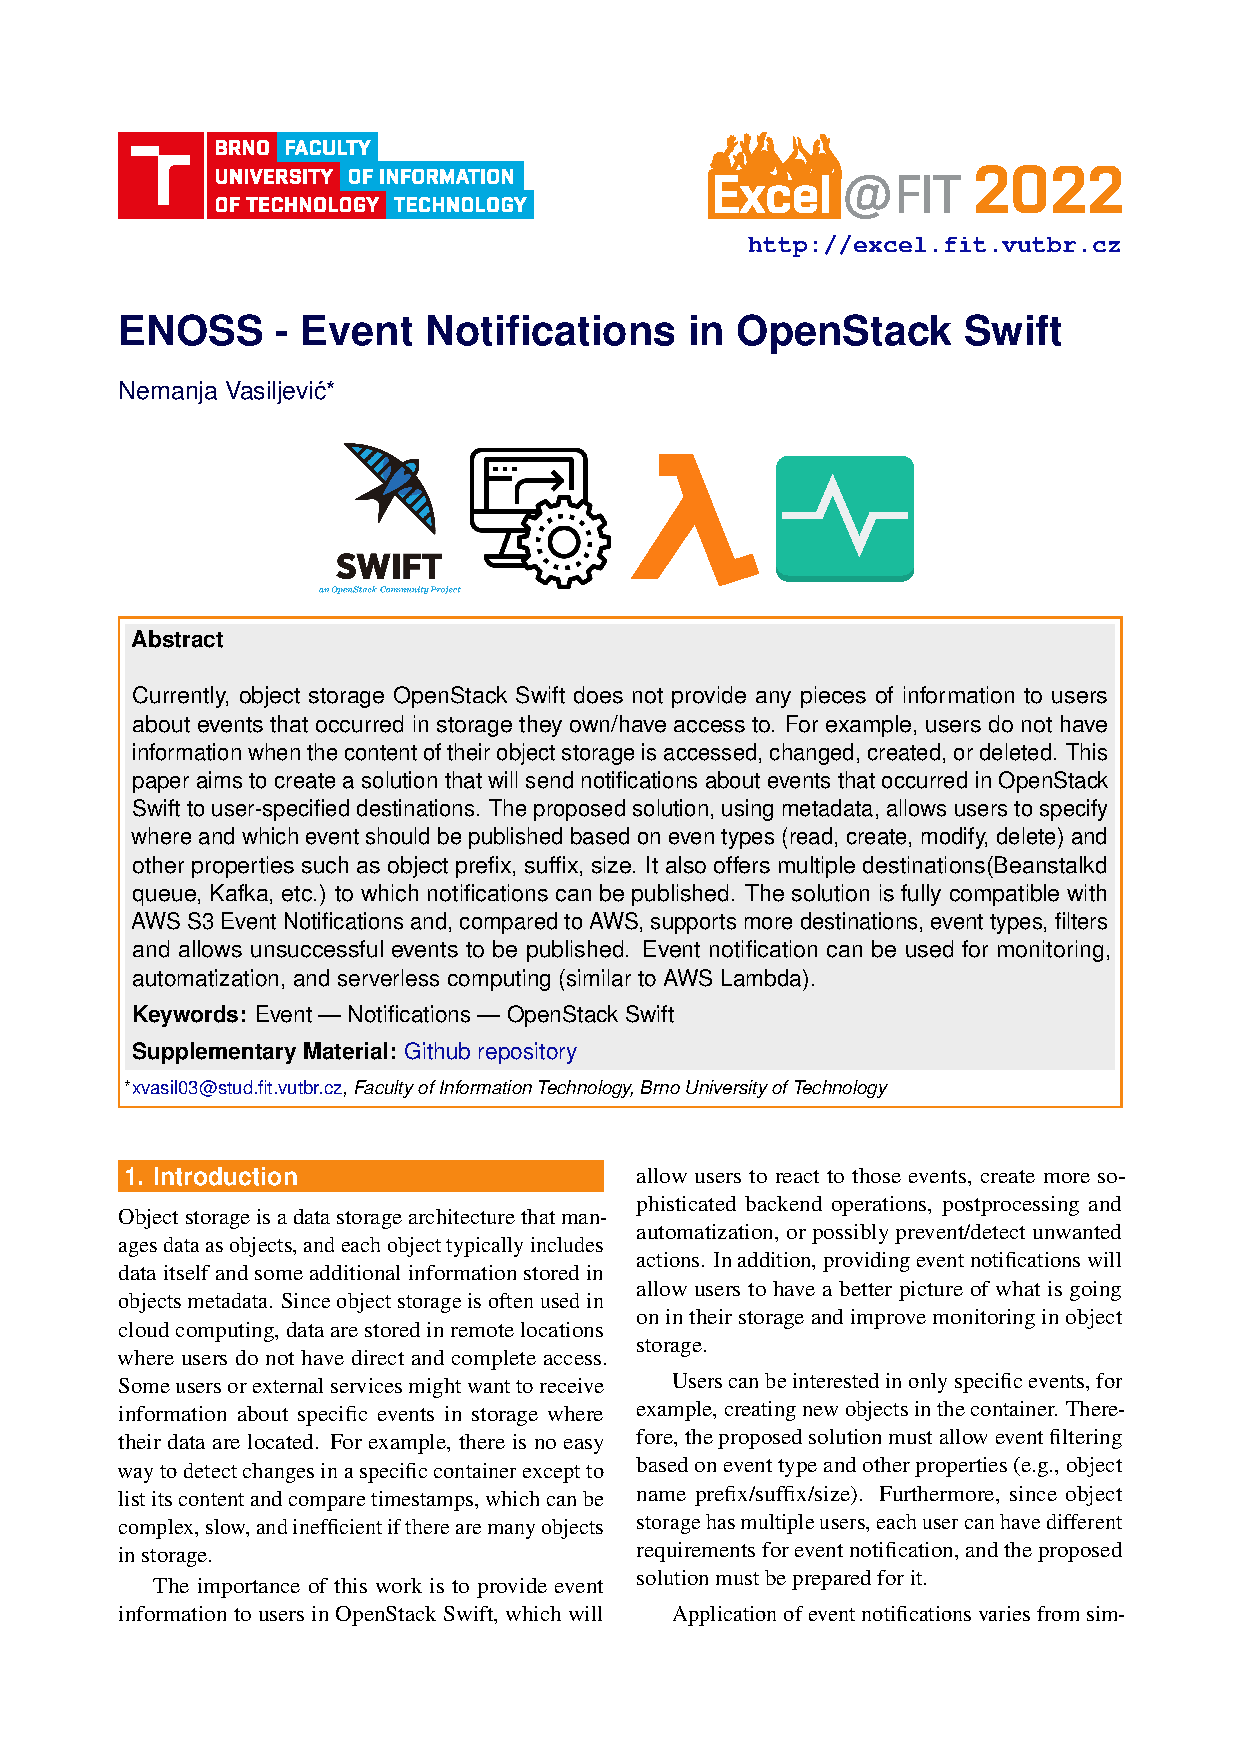
\includepdf[pages=-]{excel-paper.pdf}
